\setcounter{section}{29}
\setcounter{ex}{0}
\section{Góc giữa hai mặt phẳng trong~không~gian}
\subsection{Kiến thức cần nhớ}
\begin{khung}
\subsubsection{Góc giữa hai mặt phẳng}
	\paragraph{Khái niệm}
	\begin{itemize}
		\item Góc giữa 2 mặt phẳng là góc được tạo bởi hai đường thẳng lần lượt vuông góc với hai mặt phẳng đó.
		\item Trong không gian 3 chiều, góc giữa 2 mặt phẳng còn được gọi là \lq góc khối\rq, là phần không gian bị giới hạn bởi 2 mặt phẳng. Góc giữa 2 mặt phẳng được đo bằng góc giữa 2 đường thẳng trên mặt 2 phẳng có cùng trực giao với giao tuyến của 2 mặt phẳng.
		\end{itemize}
	\paragraph{Tính chất}
			\begin{itemize}
				\item Góc giữa 2 mặt phẳng song song bằng $ 0 $ độ;
				\item Góc giữa 2 mặt phẳng trùng nhau bằng $ 0 $ độ.
			\end{itemize}
\subsubsection{Cách xác định góc giữa 2 mặt phẳng}
Để có thể xác định chính xác góc giữa 2 mặt phẳng, chúng ta thường áp dụng những cách sau:
 
Gọi $ P $ là mặt phẳng 1, $ Q $ là mặt phẳng 2.
	\begin{itemize}
		\item \textbf{Trường hợp 1}: Hai mặt phẳng $ (P), (Q) $ song song hoặc trùng nhau thì góc của 2 mặt phẳng bằng $ 0^\circ $;
		\item \textbf{Trường hợp 2}: Hai mặt phẳng $ (P), (Q) $ không song song hoặc trùng nhau.
	\begin{itemize}
		\item \textit{Cách 1}: Dựng 2 đường thẳng $ n $ và $ p $ vuông góc lần lượt với 2 mặt phẳng $ (P) $, $ (Q) $. Khi đó góc giữa 2 mặt phẳng $ (P) $, $ (Q) $ là góc giữa 2 đường thẳng $ n $ và $ p $.
		\item \textit{Cách 2}: Để xác định góc giữa 2 mặt phẳng đầu tiên bạn cần xác định giao tuyến $ \Delta $ của 2 mặt phẳng $ (P) $ và $ (Q) $. Tiếp theo, bạn tìm một mặt phẳng $ (R) $ vuông góc với giao tuyến $ \Delta $ của 2 mặt phẳng $ (P) $, $ (Q) $ và cắt 2 mặt phẳng tại các giao tuyến $ a, b $.
		Khi đó, góc giữa 2 mặt phẳng $ (P) $, $ (Q) $ là góc giữa $ a $ và $ b $.
		\end{itemize}
	\end{itemize}
\end{khung}
\subsection{Bài tập mẫu}
\Opensolutionfile{ans}[ans/ANS-DANG-30]
\begin{khung}
	\begin{vd}[Đề tham khảo BGD 2022-2023]%[1H3B4-3] 
	\immini{Cho hình chóp $S.ABC$ có đáy là tam giác vuông tại $B$, $SA$ vuông góc với đáy và $SA=AB$ (tham khảo hình bên). Góc giữa hai mặt phẳng $(SBC)$ và $(ABC)$ bằng
	\choice[2]
	{$60^\circ$}
	{$30^\circ$}
	{$90^\circ$}
	{\True $45^\circ$}
	}{\begin{tikzpicture}[line join=round]
			\path 
			(0,0)coordinate(A)
			(-40:1)coordinate(B)
			(3,0)coordinate(C)
			(0,2.3)coordinate(S)
			;
		\foreach \x/\y/\z in {B/A/S,C/A/S}{
			\path pic[draw,angle radius=5pt]{right angle= \x--\y--\z};
		}
			\draw (S)--(A)--(B)--(S)--(C)--(B);
			\draw[dashed] (A)--(C);
			\foreach \p/\g in {A/160,B/-100,C/0,S/90}\draw[fill=white](\p) circle (0.02)node[shift={(\g:.25)}]{\footnotesize$\p$};
		\end{tikzpicture}}
	\loigiai{
	Ta có $SA\perp(ABC)$, $AB\perp BC$ nên $SB\perp BC$.\\
	Suy ra góc giữa hai mặt phẳng $(SBC)$ và $(ABC)$ bằng $\widehat{SBA}=45^\circ$ ($\triangle SAB$ vuông tại $A$ có $SA=AB$).
	}
	\end{vd}
\end{khung}
\subsection{Bài tập tương tự và phát triển}

\begin{ex}%[1H3B4-3]%[Trần Lê Nam]
\immini[thm]{Cho tứ diện $ABCD$ có $AB \perp \left(BCD \right)$. Góc giữa hai mặt phẳng $\left(ABC \right)$ và $\left(BCD \right)$ là 
\choice
{\True $90^\circ $}
{$45^\circ $}
{$60^\circ $}
{$120^\circ $}
}{%
\begin{tikzpicture}[line join=round]
			\path 
			(0,0)coordinate(A)
			(-40:1)coordinate(B)
			(3,0)coordinate(C)
			(0,2.3)coordinate(S)
			;
		\foreach \x/\y/\z in {B/A/S,C/A/S}{
			\path pic[draw,angle radius=5pt]{right angle= \x--\y--\z};
		}
			\draw (S)--(A)--(B)--(S)--(C)--(B);
			\draw[dashed] (A)--(C);
			\foreach \p/\g/\t in {A/160/B,B/-100/C,C/0/D,S/90/A}\draw[fill=white](\p) circle (0.02)node[shift={(\g:.25)}]{\footnotesize$\t$};
		\end{tikzpicture}%
}
\loigiai{
Ta có: $\heva{&AB \perp \left(BCD \right)\\
	&AB \subset \left(ABC \right)
} \Rightarrow \left(ABC \right) \perp \left(BCD \right)$.\\
Vậy góc giữa hai mặt phẳng $\left(ABC \right)$ và $\left(BCD \right)$ là $90^\circ $}
\end{ex}


\begin{ex}%[1H3B4-3]%[Trần Lê Nam]
	Gọi $\alpha $ là số đo góc giữa hai mặt phẳng $(P)$ và $(Q)$. Nếu $(P)$ và $(Q)$ song song nhau thì $\alpha $ bằng 
\choice
{$45^\circ $}
{$90^\circ $}
{$60^\circ $}
{\True $0^\circ $}
\loigiai{
A sai vì góc của hai mặt phẳng từ $0^\circ $ đến $90^\circ $.\\
B sai vì góc của hai mặt phẳng $(P)$ và $(Q)$ là $90^\circ $ thì hai mặt phẳng $(P)$ và $(Q)$ vuông góc nhau.\\
C sai vì góc của hai mặt phẳng $(P)$ và $(Q)$ là $60^\circ $ thì hai mặt phẳng $(P)$ và $(Q)$ cắt nhau.}
\end{ex}


\begin{ex}%[1H3B4-3]%[Trần Lê Nam]
	\immini[thm]{Cho hình chóp $SABC$ có $SA \perp \left(ABC \right)$ và $AB \perp BC$. Góc giữa hai mặt phẳng $(SBC)$ và $(ABC)$ là góc nào sau đây? 
\choice
{$\widehat{ASB}$}
{$\widehat{SCB}$}
{\True $\widehat{SBA}$}
{$\widehat{SCA}$}
}{\begin{tikzpicture}[line join=round]
			\path 
			(0,0)coordinate(A)
			(-40:1)coordinate(B)
			(3,0)coordinate(C)
			(0,2.3)coordinate(S)
			;
		\foreach \x/\y/\z in {B/A/S,C/A/S,C/B/A}{
			\path pic[draw,angle radius=5pt]{right angle= \x--\y--\z};
		}
			\draw (S)--(A)--(B)--(S)--(C)--(B);
			\draw[dashed] (A)--(C);
			\foreach \p/\g in {A/160,B/-100,C/0,S/90}\draw[fill=white](\p) circle (0.02)node[shift={(\g:.25)}]{\footnotesize$\p$};
		\end{tikzpicture}}
\loigiai{
Ta có: $\heva{&\left(SBC \right) \cap \left(ABC \right)=BC\\
&BC \perp AB\\
&BC \perp SB} 
\Rightarrow \left(\widehat{SB};AB \right)=\widehat{SBA}$}
\end{ex}


\begin{ex}%[1H3B4-3]%[Trần Lê Nam]
Cho hình chóp tứ giác đều $ S.ABCD $ có đáy là $ ABCD $ và độ dài các cạnh đáy bằng $ a $, $ SA = SB = SC = SD = a $. Tính $ \cos $ góc giữa hai mặt phẳng $ (SAB) $ và $ (SAD) $.
\choice
{$0$}
{\True $\dfrac{1}{3}$}
{$\dfrac{1}{2}$}
{$\dfrac{\sqrt{3}}{2}$}
\loigiai{
\immini{
Gọi $ I $ là trung điểm đoạn $ SA $. Ta có tam giác $ SAD $ và tam giác $ SAB $ đều.\\
Suy ra $ BI\perp SA$, $ DI\perp SA $.\\
Do đó, $ \left(\widehat{(SAB),(S A D)}\right)=(\widehat{B I, DI})$.\\
Áp dụng định lý cosin vào tam giác $ BID $ ta được:
\begin{eqnarray*}
\cos \widehat{BID} &&=\frac{I B^2+I D^2-B D^2}{2 \cdot I B \cdot I D}\\
&&=\dfrac{\left(\frac{\sqrt{3}}{2} a\right)^2+\left(\frac{\sqrt{3}}{2} a\right)^2-(a \sqrt{2})^2}
{2 \cdot \frac{\sqrt{3}}{2} a \cdot \frac{\sqrt{3}}{2} a}\cdot
\end{eqnarray*}
Suy ra góc $\cos\widehat{(SAB),(SAD)} = \dfrac{1}{3}\cdot$
}{
\begin{tikzpicture}[line join=round]
			\path 
			(0,0)coordinate(A)
			(-40:2)coordinate(B)
			($ (B)+(5,0) $)coordinate(C)
			($ (A)+(C)-(B)$) coordinate (D)
			(2,5) coordinate (S)
			($(A)!0.5!(S)$) coordinate (I)
			;
			\draw[dashed] (A)--(D)--(S) (I)--(D)--(B) (D)--(C);
			\draw (S)--(A)--(B)--(S)--(C)--(B)--(I);
			\foreach \p/\g in {A/180,B/-100,C/-60,S/90,I/120,D/60}\draw[fill=white](\p) circle (0.02)node[shift={(\g:.25)}]{\footnotesize$\p$};
		\end{tikzpicture}
}
}
\end{ex}


\begin{ex}%[1H3B4-3]%[Trần Lê Nam]
	Gọi $\alpha $ là số đo góc giữa hai mặt phẳng $(P)$ và $(Q)$. Nếu $(P)$ và $(Q)$ trùng nhau thì $\alpha $~bằng 
\choice
{$180^\circ $}
{$90^\circ $}
{$60^\circ $}
{\True $0^\circ $}
\loigiai{
A sai vì góc của hai mặt phẳng từ $0^\circ $ đến $90^\circ $.\\
B sai vì góc của hai mặt phẳng $(P)$ và $(Q)$ là $90^\circ $ thì hai mặt phẳng $(P)$ và $(Q)$ vuông góc nhau.\\
C vì góc của hai mặt phẳng $(P)$ và $(Q)$ là $60^\circ $ thì hai mặt phẳng $(P)$ và $(Q)$ cắt nhau}
\end{ex}


\begin{ex}%[1H3B4-3]%[Trần Lê Nam]
\immini[thm]{Cho tứ diện $ABCD$ có $AC=AD$ và $BC=BD$. Gọi $I $là trung điểm của $CD$. Khẳng định nào sau đây sai? 
\choice
{$\left(ACD \right) \perp \left(AIB \right)$}
{Góc giữa 2 mặt phẳng $\left(ACD \right)$ và $\left(BCD \right)$ là góc $\widehat{\left(AI;BI \right)}$}
{$\left(BCD \right) \perp \left(AIB \right)$}
{\True Góc giữa 2 mặt phẳng $\left(ABC \right)$ và $\left(ABD \right)$ là góc $\widehat{CBD}$}
}{\begin{tikzpicture}[line join=round]
			\path 
			(60:2) coordinate(A)
			(0,0)coordinate(B)
			(-40:1.2) coordinate(C)
			(3,0)coordinate(D)
			($ (D)!0.5!(C) $) coordinate (I)
			;
			\draw (C)--(A)--(B)--(C)--(D)--(A)--(I);
			\draw[dashed] (I)--(B)--(D);
			\foreach \p/\g in {A/90,B/100,C/-60,D/90,I/-70}\draw[fill=white](\p) circle (0.02)node[shift={(\g:.25)}]{\footnotesize$\p$};
		\end{tikzpicture}}
\loigiai{
Nếu $AB$ không vuông góc với $\left(BCD \right)$ nên góc giữa 2 mặt phẳng $\left(ABC \right)$ và $\left(ABD \right)$ không thể là góc $\widehat{CBD}$.\\
Xét đáp án B có:\\
$\left. \begin{array}{l}
CD \perp AI\\
CD \perp BI
\end{array} \right\} \Rightarrow CD \perp \left(AIB \right)$;$CD \subset \left(BCD \right)$ nên $\left(BCD \right) \perp \left(AIB \right)$. B đúng.\\
Chứng minh tương tự $\left(ACD \right) \perp \left(AIB \right)$. D đúng.\\
Xét đáp án A:\\
$\left. \begin{array}{l}
CD \perp AI\\
CD \perp BI\\
CD=\left(ACD \right) \cap \left(BCD \right)
\end{array} \right\} \Rightarrow $ 
Góc giữa 2 mặt phẳng $\left(ACD \right)$ và $\left(BCD \right)$ là góc giữa $\widehat{\left(AI;BI \right)}$.}
\end{ex}


\begin{ex}%[1H3B4-3]%[Trần Lê Nam]
\immini[thm]{Cho hình chóp $S.ABC$ có đáy $ABC$ là tam giác vuông cân tại $ A $ và $AB=a\sqrt2 $. Biết $SA \perp \left(ABC \right)$ và $SA=a$. Góc giữa hai mặt phẳng $\left(SBC \right)$ và $\left(ABC \right)$ bằng 
\choice
{$ 60^\circ $}
{$ 90^\circ $}
{\True $ 45^\circ $}
{$ 30^\circ $}
}{\begin{tikzpicture}[line join=round]
			\path 
			(60:2) coordinate(A)
			(0,0)coordinate(B)
			(-40:1.2) coordinate(C)
			(3,0)coordinate(D)
			($ (D)!0.5!(C) $) coordinate (M)
			;
			\draw (C)--(A)--(B)--(C)--(D)--(A)--(M);
			\draw[dashed] (M)--(B)--(D);
			\foreach \p/\g/\t in {A/90/S,B/100/A,C/-60/B,D/90/C,M/-70/M}\draw[fill=white](\p) circle (0.02)node[shift={(\g:.25)}]{\footnotesize$\t$};
		\end{tikzpicture}}
\loigiai{
Trong mặt phẳng $\left(ABC \right)$ kẻ $AM \perp BC$ tại $M$.\\
Ta có $\heva{&\left(SBC \right) \cap \left(ABC \right)=BC\\
	&\left(SAM \right) \perp BC\\
	&\left(SAM \right) \cap \left(SBC \right)=SM\\
	& \left(SAM \right) \cap \left(ABC \right)=AM}
\Rightarrow \widehat{\left(SBC \right),\left(ABC \right)}=\left(\widehat{SM,AM}\right)$.\\
Suy ra góc giữa $\left(SBC \right)$ và $\left(ABC \right)$ bằng góc $\widehat{SMA}$.\\
Xét tam giác $ABC$ ta có $BC=AB.\sqrt 2=a\sqrt 2.\sqrt 2=2a \Rightarrow AM=\dfrac{1}{2}BC=a$.\\
Xét tam giác $SAM$ vuông tại $A$ ta có $\tan \widehat{SMA}=\dfrac{SA}{AM}=\dfrac{a}{a}=1 \Rightarrow \widehat{SMA}=45^\circ $.
}
\end{ex}


\begin{ex}%[1H3B4-3]%[Trần Lê Nam]
\immini[thm]{Cho hình lăng trụ đều $ABC.A'B'C'$ có cạnh đáy bằng $2a$, cạnh bên bằng $a$. Tính góc giữa hai mặt phẳng $\left(AB'C' \right)$ và $\left(A'B'C' \right)$. 
\choice
{$\dfrac{\pi}{2}$}
{$\dfrac{3\pi}{2}$}
{\True$\dfrac{\pi}{6}$}
{$\dfrac{\pi}{3}$}
}{
  \begin{tikzpicture}[declare function={a=3;b=-1;h=2;},line join=round]
	  \foreach \x/\y/\z in {0/0/A,h/b/B,a/0/C,0/h/{A'},h/{b+h}/{B'},a/{h}/{C'},
	  }{
	      \path (\x,\y) coordinate (\z);
	  }
	  \path ($ (B')!0.5!(C') $) coordinate (I);
	  \draw[dashed] (I)--(A)--(C) (C')--(A)--(B');
	  \draw (B)--(B') (I)--(A')--(C') (A)--(B)--(C)--(C')--(B')--(A')--cycle;
	  \foreach \t/\g in {A/180,B/-90,C/0,A'/180,B'/-20,C'/0,I/90}{
	  	\draw[fill=white] (\t) circle (1pt) node[shift={(\g:7pt)},font=\scriptsize]{$ \t $};
	  }
  \end{tikzpicture}
}
\loigiai{%
Gọi $I$ là trung điểm của $ B’C’ $ ta có $\heva{&AI \perp B'C'\\
	&A'I \perp B'C'} \Rightarrow \left(\left(AB'C' \right);\left(A'B'C' \right) \right)=\widehat{\left(AI;A'I \right)}=\widehat{AIA'}.$\\
Xét tam giác $AIA'$ vuông tại $A'$ ta có: $\tan \widehat{AIA'}=\dfrac{AA'}{A'I}=\dfrac{a}{a\sqrt 3}=\dfrac{1}{\sqrt 3}$ \\
 $ \Rightarrow \widehat{AIA'}=\widehat{\left(\left(AB'C' \right),\left(ABC \right) \right)}=\dfrac{\pi}{6}$.
}
\end{ex}



\begin{ex}%[1H3B4-3]%[Trần Lê Nam]
\immini[thm]{Cho hình chóp $S.ABC$ có tam giác $ABC$ vuông cân tại $B$, $AB=BC=a$, $SA=a\sqrt 3 $, $SA \perp \left(ABC \right)$. Góc giữa hai mặt phẳng $\left(SBC \right)$và $\left(ABC \right)$ là 
\choice
{\True $60^\circ $}
{$90^\circ $}
{$30^\circ $}
{$45^\circ $}
}{
\begin{tikzpicture}[line join=round]
			\path 
			(0,0)coordinate(A)
			(-40:1)coordinate(B)
			(3,0)coordinate(C)
			(0,2.3)coordinate(S)
			;
		\foreach \x/\y/\z in {B/A/S,C/A/S,C/B/A}{
			\path pic[draw,angle radius=5pt]{right angle= \x--\y--\z};
		}
			\draw (S)--(A)--(B)--(S)--(C)--(B);
			\draw[dashed] (A)--(C);
			\foreach \p/\g in {A/160,B/-100,C/0,S/90}\draw[fill=white](\p) circle (0.02)node[shift={(\g:.25)}]{\footnotesize$\p$};
		\end{tikzpicture}
}
\loigiai{%
Ta có $BC \perp \left(SAB \right) \Rightarrow BC \perp SA$.\\ Góc giữa hai mặt phẳng $\left(SBC \right)$ và $\left(ABC \right)$ là góc $\widehat{SBA}$. \\
$\tan \widehat{SBA}=\dfrac{SA}{AB}=\dfrac{a\sqrt 3}{a}=\sqrt 3 $\\
$ \Rightarrow \widehat{SBA}=60^\circ $.}
\end{ex}


\begin{ex}%[1H3B4-3]%[Trần Lê Nam]
\immini[thm]{Cho hình chóp $S.ABC$ có cạnh $SA$ vuông góc với mặt phẳng $\left(ABC \right)$, biết $AB=AC=a$, $BC=a\sqrt 3 $. Tính góc giữa hai mặt phẳng $\left(SAB \right)$ và $\left(SAC \right)$. 
\choice
{\True $60^\circ $}
{$45^\circ $}
{$30^\circ $}
{$90^\circ $}
}{
\begin{tikzpicture}[line join=round]
			\path 
			(0,0)coordinate(A)
			(-40:1)coordinate(B)
			(3,0)coordinate(C)
			(0,2.3)coordinate(S)
			;
		\foreach \x/\y/\z in {B/A/S,C/A/S}{
			\path pic[draw,angle radius=5pt]{right angle= \x--\y--\z};
		}
			\draw (S)--(A)--(B)--(S)--(C)--(B);
			\draw[dashed] (A)--(C);
			\foreach \p/\g in {A/160,B/-100,C/0,S/90}\draw[fill=white](\p) circle (0.02)node[shift={(\g:.25)}]{\footnotesize$\p$};
		\end{tikzpicture}
}
\loigiai{
Vì $SA \perp \left(ABC \right)$ nên $SA \perp AB$ và $SA \perp AC$.\\
Ta có: $\heva{&\left(SAB \right) \cap \left(SAC \right)=SA\\
	& SA \perp AB\\
	& SA \perp AC} 
\Rightarrow \widehat{\left(SAB \right),\left(SAC \right)}=\widehat{\left(AB,AC \right)}$.\\
Xét $\triangle ABC$ có $\cos \widehat{BAC}=\dfrac{AB^2 + AC^2 - BC^2}{2.AB.AC}=\dfrac{a^2 + a^2 - \left(a\sqrt 3 \right)^2}{2.a.a}=- \dfrac{1}{2}\Rightarrow \widehat{BAC}=120^\circ $.\\
Vậy $\widehat{\left(SAB \right),\left(SAC \right)}=180^\circ - \widehat{BAC} = 180^\circ - 120^\circ = 60^\circ$.
}
\end{ex}


\begin{ex}%[1H3B4-3]%[Trần Lê Nam]
\immini[thm]{Cho hình chóp $S.ABC$ có đáy là tam giác đều cạnh $a$, $SA \perp \left(ABC \right)$, góc giữa hai mặt phẳng $\left(ABC \right)$ và $\left(SBC \right)$ là $60^\circ$. Độ dài cạnh $SA$ bằng 
\choice
{$\dfrac{a}{\sqrt 3}$}
{$\dfrac{a}{2}$}
{$a\sqrt 3 $}
{\True $\dfrac{3a}{2}$}
}{
\begin{tikzpicture}[line join=round]
			\path 
			(0,0)coordinate(A)
			(-40:1)coordinate(B)
			(3,0)coordinate(C)
			(0,2.3)coordinate(S)
			;
		\foreach \x/\y/\z in {B/A/S,C/A/S}{
			\path pic[draw,angle radius=5pt]{right angle= \x--\y--\z};
		}
			\draw (S)--(A)--(B)--(S)--(C)--(B);
			\draw[dashed] (A)--(C);
			\foreach \p/\g in {A/160,B/-100,C/0,S/90}\draw[fill=white](\p) circle (0.02)node[shift={(\g:.25)}]{\footnotesize$\p$};
		\end{tikzpicture}
}
\loigiai{%
Gọi $I$ là trung điểm $BC$, khi đó $BC \perp AI$.\\
Mặt khác $BC \perp AI,\,BC \perp SA \Rightarrow BC \perp \left(SAI \right) \Rightarrow BC \perp SI$.\\
Suy ra góc giữa hai mặt phẳng $\left(ABC \right)$ và $\left(SBC \right)$ là $\widehat{SIA}$.\\
Tam giác $SIA$ vuông tại $A$ nên $\tan \widehat{SIA}=\dfrac{SA}{AI} \Leftrightarrow SA=IA.\tan \widehat{SIA}=\dfrac{a\sqrt 3}{2}.\sqrt 3=\dfrac{3a}{2}$.}
\end{ex}


\begin{ex}%[1H3B4-3]%[Trần Lê Nam]
\immini[thm]{Cho tứ diện $OABC$ có $OA$, $OB$, $OC$ đôi một vuông góc và $OB=OC=a\sqrt 6 $, $OA=a$. Tính góc giữa hai mặt phẳng $\left(ABC \right)$ và $\left(OBC \right)$. 
\choice
{$90^\circ $}
{$60^\circ $}
{\True $30^\circ $}
{$45^\circ $}
}{
\begin{tikzpicture}[line join=round]
			\path 
			(0,0) coordinate(O)
			(90:2) coordinate(A)
			(220:1.5)coordinate(B)
			(0:2.5)coordinate (C)
			;
		\foreach \x/\y/\z in {A/O/B,C/O/A,B/O/C}{
			\path pic[draw,angle radius=5pt]{right angle= \x--\y--\z};
		}
		\draw[dashed] (A)--(O)--(B) (O)--(C);
			\draw (A)--(B)--(C)--(A);
			\foreach \p/\g in {A/90,B/-90,C/0,O/-50}\draw[fill=white](\p) circle (0.02)node[shift={(\g:.25)}]{\footnotesize$\p$};
		\end{tikzpicture}
}
\loigiai{
Gọi $I$ là trung điểm của $BC \Rightarrow AI \perp BC$.
 Mà $OA \perp BC$ nên $AI \perp BC$.\\
Ta có: $\heva{&\left(OBC \right) \cap \left(ABC \right)=BC\\
	&BC \perp AI\\
	&BC \perp OI} \Rightarrow \widehat{\left(OBC \right),\left(ABC \right)}=\widehat{\left(OI,AI \right)}=\widehat{OIA}$.\\
Ta có: $OI=\dfrac{1}{2}BC=\dfrac{1}{2}\sqrt{OB^2 + OC^2}=a\sqrt 3 $.\\
Xét tam giác $OAI$ vuông tại $A$ có $\tan \widehat{OIA}=\dfrac{OA}{OI}=\dfrac{\sqrt 3}{3} \Rightarrow \widehat{OIA}=30^\circ $.\\
Vậy $\widehat{\left(OBC \right),\left(ABC \right)}=30^\circ $.}
\end{ex}


\begin{ex}%[1H3B4-3]%[Trần Lê Nam]
\immini[thm]{Cho hình chóp $S.ABC$ có cạnh $SA$ vuông góc với mặt phẳng $\left(ABC \right)$, biết $AB=AC=a$, $BC=a\sqrt 3 $. Tính góc giữa hai mặt phẳng $\left(SAB \right)$ và $\left(SAC \right)$.  
\choice
{\True $60^\circ $}
{$150^\circ $}
{$30^\circ $}
{$120^\circ $}
}{%
\begin{tikzpicture}[line join=round]
			\path 
			(0,0)coordinate(A)
			(-40:1)coordinate(B)
			(3,0)coordinate(C)
			(0,2.3)coordinate(S)
			;
		\foreach \x/\y/\z in {B/A/S,C/A/S}{
			\path pic[draw,angle radius=5pt]{right angle= \x--\y--\z};
		}
			\draw (S)--(A)--(B)--(S)--(C)--(B);
			\draw[dashed] (A)--(C);
			\foreach \p/\g in {A/160,B/-100,C/0,S/90}\draw[fill=white](\p) circle (0.02)node[shift={(\g:.25)}]{\footnotesize$\p$};
		\end{tikzpicture}
}
\loigiai{
Ta có: $\heva{&AB \perp SA, AB \subset \left(SAB \right)\\
	&AC \perp SA, AC \subset \left(SAC \right)\\
	&\left(SAB \right) \cap \left(SAC \right)=SA} \Rightarrow \widehat{\left(\left(SAB \right),\left(SAC \right) \right)}=\left(AB,AC \right)$.\\
Xét tam giác $ABC$ ta có: $\cos \widehat{BAC}=\dfrac{AB^2 + AC^2 - BC^2}{2AB.AC}=\dfrac{a^2 + a^2 - 3a^2}{2.a.a}=- \dfrac{1}{2}$ \\
$\Rightarrow \widehat{BAC}=120^\circ $.\\
Vậy $\widehat{\left(\left(SAB \right),\left(SAC \right) \right)}=\left(AB,AC \right)=180^\circ - 120^\circ=60^\circ $.}
\end{ex}


\begin{ex}%[1H3B4-3]%[Trần Lê Nam]
\immini[thm]{Cho hình chóp $S.ABC$có $SA \perp \left(ABC \right)$
	và $AB \perp BC$, gọi $I$là trung điểm $BC$. Góc giữa hai mặt phẳng $\left(SBC \right)$và $\left(ABC \right)$ là góc nào sau đây? 
\choice
{$\widehat{SIA}$}
{\True$\widehat{SBA}$}
{$\widehat{SCA}$}
{$\widehat{SCB}$}
}{
\begin{tikzpicture}[line join=round]
			\path 
			(0,0)coordinate(A)
			(-40:1)coordinate(B)
			(3,0)coordinate(C)
			(0,2.3)coordinate(S)
			;
		\foreach \x/\y/\z in {B/A/S,C/A/S,C/B/A}{
			\path pic[draw,angle radius=5pt]{right angle= \x--\y--\z};
		}
			\draw (S)--(A)--(B)--(S)--(C)--(B);
			\draw[dashed] (A)--(C);
			\foreach \p/\g in {A/160,B/-100,C/0,S/90}\draw[fill=white](\p) circle (0.02)node[shift={(\g:.25)}]{\footnotesize$\p$};
		\end{tikzpicture}
}
\loigiai{
$\left(SBC \right) \cap \left(ABC \right)=BC$; $BC \perp BA;BC \perp SA$nên $BC \perp \left(SAB \right)$\\
Vậy $\widehat{\left(\left(SBC \right);\left(ABC \right) \right)}=\widehat{\left(SB;AB \right)}=\widehat{SBA}$}
\end{ex}


\begin{ex}%[1H3B4-3]%[Trần Lê Nam]
\immini[thm]{Cho hình chóp tam giác đều có cạnh đáy bằng $a$. Góc giữa cạnh bên và mặt đáy bằng $60^\circ $ (tham khảo hình vẽ bên). Cosin của góc giữa mặt bên và mặt đáy của hình chóp là. 
\choice
{\True$\dfrac{1}{\sqrt 13}$}
{$\dfrac{1}{2\sqrt 3}$}
{$\dfrac{2\sqrt 3}{\sqrt 13}$}
{$\dfrac{1}{\sqrt 3}$}
}{%
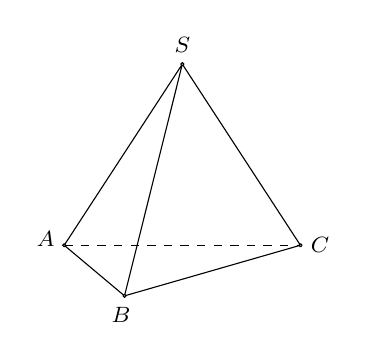
\begin{tikzpicture}[line join=round]
			\path 
			(0,0)coordinate(A)
			(-40:1)coordinate(B)
			(3,0)coordinate(C)
			(1.5,2.3)coordinate(S)
			;
			\draw (S)--(A)--(B)--(S)--(C)--(B);
			\draw[dashed] (A)--(C);
			\foreach \p/\g in {A/160,B/-100,C/0,S/90}\draw[fill=white](\p) circle (0.02)node[shift={(\g:.25)}]{\footnotesize$\p$};
		\end{tikzpicture}
}
\loigiai{Gọi $M$ là trung điểm cạnh $BC$và $O$là tâm đường tròn ngoại tiếp tam giác $ABC$.\\
Góc giữa cạnh bên $SA$và mặt đáy $\left(ABC \right)$ là $60^\circ$.\\
$ \Rightarrow \widehat{SAO}=60^\circ \Rightarrow SO=OA.\tan 60^\circ=\dfrac{a\sqrt 3}{3}.\sqrt 3=a$.\\
Góc giữa mặt bên $\left(SBC \right)$ và mặt đáy $\left(ABC \right)$là $\widehat{SMO}$.\\
Ta có $\cos\widehat{SMO}=\dfrac{OM}{SM}=\dfrac{OM}{\sqrt SO^2 + OM^2}=\dfrac{\dfrac{a\sqrt 3}{6}}{\sqrt a^2 + \left(\dfrac{a\sqrt 3}{6} \right)^2}=\dfrac{1}{\sqrt 13}$.}
\end{ex}


\begin{ex}%[1H3B4-3]%[Trần Lê Nam]
\immini[thm]{Cho tứ diện đều $ABCD$. Cosin của góc giữa hai mặt phẳng $\left(ABC \right)$ và $\left(DBC \right)$ bằng 
\choice
{$\dfrac{\sqrt 3}{2}$}
{$\dfrac{\sqrt 2}{2}$}
{$\dfrac{1}{2}$}
{\True$\dfrac{1}{3}$}
}{%
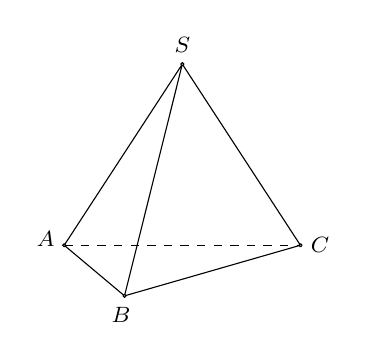
\begin{tikzpicture}[line join=round]
			\path 
			(0,0)coordinate(A)
			(-40:1)coordinate(B)
			(3,0)coordinate(C)
			(1.5,2.3)coordinate(S)
			;
			\draw (S)--(A)--(B)--(S)--(C)--(B);
			\draw[dashed] (A)--(C);
			\foreach \p/\g in {A/160,B/-100,C/0,S/90}\draw[fill=white](\p) circle (0.02)node[shift={(\g:.25)}]{\footnotesize$\p$};
		\end{tikzpicture}
}
\loigiai{
Gọi tứ diện $ABCD$ là tứ diện đều cạnh $ a $.\\
Gọi $H$ là tâm của tam giác$ABC$. Khi đó $DH \perp \left(ABC \right)$ tại $H$.\\
Gọi $I$ là trung điểm của $BC$. Khi đó góc giữa mặt phẳng $\left(DBC \right)$ và $\left(ABC \right)$ là góc $\widehat{DIH}$\\
Ta có $\cos \widehat{\left(\left(ABC \right),\left(DBC \right) \right)}=\cos \widehat{DIH}=\dfrac{IH}{ID}$.\\
Tam giác $ABC$ đều $ \Rightarrow IH=\dfrac{1}{3}IA=\dfrac{1}{3}.\dfrac{a\sqrt 3}{2}=\dfrac{a\sqrt 3}{6}$.\\
Tam giác $DBC$ đều $ \Rightarrow ID=\dfrac{a\sqrt 3}{2} \Rightarrow \cos \widehat{\left(\left(ABC \right),DBC \right)}=\dfrac{1}{3}$.}
\end{ex}


\begin{ex}%[1H3B4-3]%[Trần Lê Nam]
\immini[thm]{Cho khối chóp $S.ABC$ có mặt đáy $ABC$ là tam giác cân tại $A$ với $BC=2a$, góc $\widehat{BAC}=120^\circ $. Biết cạnh bên $SA$ vuông góc với mặt đáy và thể tích khối chóp $S.ABC$ bằng $\dfrac{a^3}{9}$. Tính góc hợp bởi mặt phẳng $\left(SBC \right)$ và mặt phẳng đáy. 
\choice
{\True$45^\circ $}
{$60^\circ $}
{$30^\circ $}
{$90^\circ $}
}{%
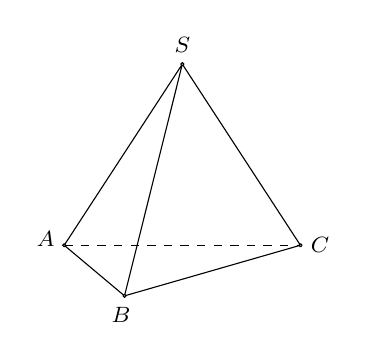
\begin{tikzpicture}[line join=round]
			\path 
			(0,0)coordinate(A)
			(-40:1)coordinate(B)
			(3,0)coordinate(C)
			(1.5,2.3)coordinate(S)
			;
			\draw (S)--(A)--(B)--(S)--(C)--(B);
			\draw[dashed] (A)--(C);
			\foreach \p/\g in {A/160,B/-100,C/0,S/90}\draw[fill=white](\p) circle (0.02)node[shift={(\g:.25)}]{\footnotesize$\p$};
		\end{tikzpicture}
}
\loigiai{
Gọi $I$ là trung điểm $BC$, xét tam giác $AIB$ vuông tại $I$ ta có:\\
$\tan 60^\circ=\sqrt 3=\dfrac{BI}{AI} \Leftrightarrow AI=\dfrac{a\sqrt 3}{3}$ (Do góc $BAI=60^\circ $, $AI$ là phân giác góc $120^\circ $)\\
$S_{\triangle ABC}=\dfrac{1}{2}AI.BC=\dfrac{1}{2}.\dfrac{a\sqrt 3}{3}.2a=\dfrac{a^2\sqrt 3}{3}$\\
Do đó $V_{SABC}=\dfrac{1}{3}SA.S_{\triangle ABC}=\dfrac{a^3}{9} \Leftrightarrow SA=\dfrac{a\sqrt 3}{3}$\\
Mà $\left\{\begin{array}{l}
BC \perp AI\\
BC \perp SA
\end{array} \right. \Rightarrow BC \perp \left(SAI \right) \Rightarrow BC \perp SI$.\\
Vậy góc hợp bởi mặt phẳng $\left(SBC \right)$ và mặt phẳng đáy là góc $\widehat{SIA}$.\\
Suy ra tam giác $SIA$ vuông cân tại $A$ nên $\widehat{SIA}=45^\circ $}
\end{ex}

\begin{ex}%[1H3B4-3]%[Trần Lê Nam]
	Cho hình lập phương $ABCD.A'B'C'D'$. Góc giữa hai mặt phẳng $\left(A'AC \right)$ và $\left(ABCD \right)$ bằng
\choice
{\True$90^\circ$}
{$60^\circ$}
{$30^\circ$}
{$45^\circ$}
\loigiai{
\immini{
Vì $AA' \perp \left(ABCD \right)$ nên $\left(A'AC \right) \perp \left(ABCD \right)$.\\
Do đó góc giữa hai mặt phẳng $\left(A'AC \right)$ và $\left(ABCD \right)$ bằng $90^\circ$.}
{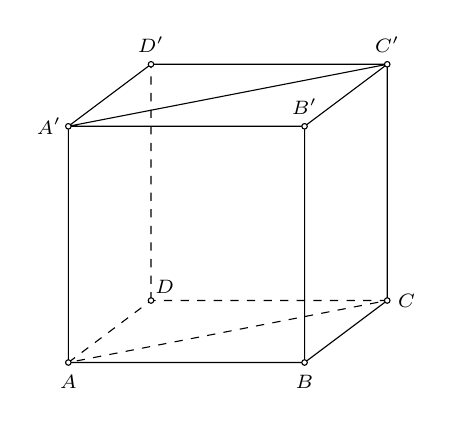
\begin{tikzpicture}[declare function={a=3;b=0.35*a;c=0.75*b;},line join=round]
	  \foreach \x/\y/\z in {0/0/A,a/0/B,{a+b}/c/C,b/c/D,0/a/A',a/{a}/B',{a+b}/{c+a}/C',b/{c+a}/D',
	  }{
	      \path (\x,\y) coordinate (\z);
	  }
	  \draw[dashed] (D)--(D') (A)--(D)--(C)--cycle;
	  \draw  (C')--(C)--(B) (A')--(C')
	  (A')--(A)--(B)--(B')--(A')--(D')--(C')--(B');
	  \foreach \t/\g in {A/-90,B/-90,C/0,D/45,A'/180,B'/90,C'/90,D'/90}{
	  	\draw[fill=white] (\t) circle (1pt) node[shift={(\g:7pt)},font=\scriptsize]{$ \t $};
	  }
  \end{tikzpicture}}
  }
\end{ex}
\begin{ex}%[1H3B4-3]%[Trần Lê Nam]
	Cho hình lập phương $ABCD.A'B'C'D'$. Góc giữa hai mặt phẳng $\left(ADD'A' \right)$ và $\left(ABC'D' \right)$~bằng
\choice
{$60^\circ $}
{$45^\circ $}
{\True$90^\circ $}
{$30^\circ $}
\loigiai{
\immini{
Ta có $AB \perp \left(ADD'A' \right)$, suy ra $\left(ABC'D' \right) \perp \left(ADD'A' \right)$.\\
 Do đó, $\widehat{\left(ADD'A' \right),\left(ABC'D' \right)}= 90^\circ $.}{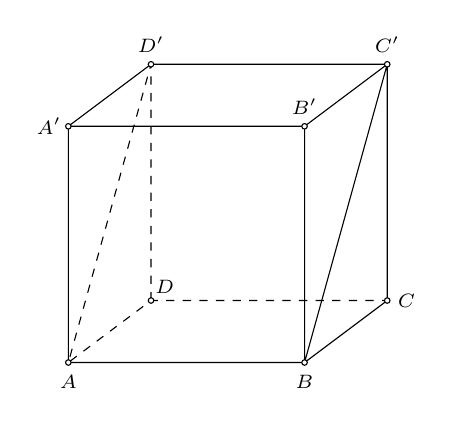
\begin{tikzpicture}[declare function={a=3;b=0.35*a;c=0.75*b;},line join=round]
	  \foreach \x/\y/\z in {0/0/A,a/0/B,{a+b}/c/C,b/c/D,0/a/A',a/{a}/B',{a+b}/{c+a}/C',b/{c+a}/D',
	  }{
	      \path (\x,\y) coordinate (\z);
	  }
	  \draw[dashed] (D)--(D')--(A)--(D)--(C);
	  \draw  (C')--(C)--(B) (B)--(C')
	  (A')--(A)--(B)--(B')--(A')--(D')--(C')--(B');
	  \foreach \t/\g in {A/-90,B/-90,C/0,D/45,A'/180,B'/90,C'/90,D'/90}{
	  	\draw[fill=white] (\t) circle (1pt) node[shift={(\g:7pt)},font=\scriptsize]{$ \t $};
	  }
  \end{tikzpicture}}
  }
\end{ex}

\begin{ex}%[1H3B4-3]%[Trần Lê Nam]
	Cho hình lập phương $ABCD.A'BC'D'$. Tính góc giữa mặt phẳng $\left(ABB'A' \right)$ và $\left(ABC'D' \right)$.
\choice
{$30^\circ $}
{$90^\circ $}
{\True$45^\circ $}
{$60^\circ $}
\loigiai{ 
\begin{center}
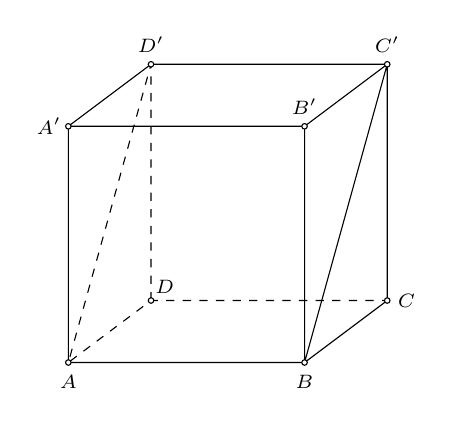
\begin{tikzpicture}[declare function={a=3;b=0.35*a;c=0.75*b;},line join=round]
	  \foreach \x/\y/\z in {0/0/A,a/0/B,{a+b}/c/C,b/c/D,0/a/A',a/{a}/B',{a+b}/{c+a}/C',b/{c+a}/D',
	  }{
	      \path (\x,\y) coordinate (\z);
	  }
	  \draw[dashed] (D)--(D')--(A)--(D)--(C);
	  \draw  (C')--(C)--(B) (B)--(C')
	  (A')--(A)--(B)--(B')--(A')--(D')--(C')--(B');
	  \foreach \t/\g in {A/-90,B/-90,C/0,D/45,A'/180,B'/90,C'/90,D'/90}{
	  	\draw[fill=white] (\t) circle (1pt) node[shift={(\g:7pt)},font=\scriptsize]{$ \t $};
	  }
  \end{tikzpicture}
\end{center}
Ta có
\begin{align*}
	\left.
		\begin{array}{l}
			(ABB'A')\cap (ABC'D')=AB\\
			AB\perp (BCC'B')\\
			(ABB'A')\cap (BCC'B')=BB'\\
			(ABC'D')\cap (BCC'B')=BC'
		\end{array}
	\right\}
	\Rightarrow
	\widehat{\left(ABB'A' \right),\left(ABC'D' \right)}
	=\widehat{C'BB'}=45^\circ.
\end{align*}
  }
\end{ex}
\Closesolutionfile{ans}
%======================
\subsection{Bảng đáp án}
\inputansbox{8}{ans/ANS-DANG-30}